\ifpdf
    \graphicspath{{Chapter7/Figs/Raster/}{Chapter7/Figs/PDF/}{Chapter7/Figs/}}
\else
    \graphicspath{{Chapter7/Figs/Vector/}{Chapter7/Figs/}}
\fi


\chapter[State of the Art White Supremacy: On Disembodiment in the Machine Learning Pipeline]{State of the Art White Supremacy: On Disembodiment in the Machine Learning Pipeline\footnotemark{}}\label{chap:disembodied}
\chaptermark{State of the Art White Supremacy}
\footnotetext{This chapter contains elements from a collaboration with Smarika Lulz, Joachim Bingel, and Isabelle Augenstein. The associated paper is currently under review in the Conference on Fairness, Accountability, and Transparancy (FAccT). The title is taken from a conversation between Abeba Birhane, Chris Dancy and myself, where Chris offered the term State-of-the-Art White Supremacy.}

\begin{citequote}{\citet[p.110-111]{Lorde:1984}}
What does it mean when the tools of a racist patriarchy are used to examine the fruits of that same patriarchy?  It means that only the most narrow parameters of change are possible and allowable.
\end{citequote}

In the previous chapters we have identified different areas of concern for the use of models and data. \ZTedit{From the ways in which content moderation technologies come to create discriminatory outcomes in \autoref{chap:filter}, to the
\ZTdelete{From the} constraints of document transformation in \autoref{chap:LIWC}, and the influence of multiple data sources and prediction tasks in \autoref{chap:mtl}.
In these chapters, I sought to find means to \ZTedit{contextualise computational methods, and to} make \ZTdelete{computational methods}\ZTedit{them} more closely \ZTdelete{come to} represent the subjectivities and contexts of speakers from within frames of existing computational methods.
As the chapters collectively point to, there is an inherent limitation to what is achievable within computational pipelines in which the entire process, from dataset creation to modelling, is not developed while respecting human subjectivities.
\ZTedit{More precisely}\ZTdelete{Specifically}, the need for finding ways to approximate contexts and subjectivities highlights how the current machine learning pipeline does not specify how subjectivities are embedded in these technologies.
Understanding precisely where such shortcomings arise in the machine learning pipeline requires a deeper consideration of \ZTedit{machine learning and the} human embodiments within \ZTdelete{it}\ZTedit{the pipeline}.
Moreover, it requires a deeper consideration of how machine learning, as an academic practice, presents itself and disembodies itself from the subjective human experiences that machine learning purports to be developed for.
For this reason, I turn to considering how \ZTedit{the machine learning pipeline embodies and disembodies human (experience).}\ZTdelete{human embodiment and disembodiment happens throughout the machine learning pipeline.}
\ZTdelete{Here}\ZTedit{Therefore}, I return to \textit{RQ I} by asking how subjective experiences are embodied in the machine learning pipeline (\textit{RQ 4}) and what the implications of this are (\textit{RQ 5}).
In this chapter, I \ZTdelete{then} theorise \ZTdelete{over}\ZTedit{on} the core sources of these issues: the context within which models and exist, the models and the data.
To describe these issues, I invoke the metaphor of the body in three different ways: first, pertaining to the physical material \textit{human body} that we each possess; second, to signify a collection of observations and data points \textit{created by humans}; and third, to refer subjective embodiments, that is how \textit{social and cultural meaning} is embedded in the human experience and derivatives of it, i.e. data created by humans.
I then \ZTedit{reflexively} apply my theory  to the computational models in \cref{chap:LIWC,chap:mtl} and \ZTdelete{apply}\ZTedit{provide} a critique of these technologies through a consideration of the data generation process and the modelling stages of the machine learning pipeline.
Finally, I discuss the implications of current practices in machine learning and argue that \ZTedit{we must radically reconsider our current approaches to machine learning for social tasks, such that our approaches align better with the stated aims.}\ZTdelete{for machine learning for social prediction tasks to achieve their goals, we must radically reconsider current approaches to better align with the stated aims.}

\section{Disembodied Machine Learning}
Machine learning is a practice that is concerned with making decisions based on machine-discernible patterns in observed data.
Often, the data used to optimise machine learning methods are `extracted' from the context within which they are created, i.e. by `scraping' online platforms for user-generated content.
Through this process of separating context and datum, a notion of `objectivity' is imposed upon the data and the subsequent operations, \ZTdelete{i.e.}\ZTedit{namely,} optimising machine learning methods on the data and their results further entrench this notion \ZTedit{of objectivity}.
Datasets, or bodies of data, are thus created through \ZTdelete{a repeated}\ZTedit{the repetition of separating}\ZTdelete{separation of} datum from context.
These amalgamated bodies of data exist only by virtue of their strict separation from the material bodies from which the datum are derived.
\ZTdelete{These}\ZTedit{Such} disembodied and amalgamated bodies are then used to optimise machine learning models.
Machine learning methods come in two different forms: Supervised learning methods which seek to distinguish distinct limbs which are pre-drawn, e.g. classes, from the data; and unsupervised models which seek to identify discernible limbs of data within a single body of data without direct guidance from designers.
For both supervised and unsupervised models the underlying data and the models applied to them \ZTdelete{have strong influences as to}\ZTedit{strongly influence} what bodies are discovered and what may be \ZTdelete{discovered}\ZTedit{uncovered} within these data.
As \citet{Benjamin:2019} writes, technology operates within social structure ``codes [that] operate within powerful systems of meaning that render some things visible, others invisible, and creates a vast array of distortions and dangers''.\vspace{5mm}

With the advent of machine learning, a new technology came to be hailed as objective and unimpeded by subjective human biases, and by extension social marginalisation \citep{oneil:2017}.
However, an increasing amount of research suggests that social biases are common to machine learning models \citep{Shah:2020,Buolamwini:2018,Agarwal:2018}.
Moreover, research has found that biases in the underlying data may be exacerbated by the machine learning models \citep{Zhao:2017,Jia:2020}.
As a result of this growing awareness of the emergence of social biases in machine learning models, there has been a number of research directions seek to identify \citep{Shah:2020,Bender-Friedman:2018,Mitchell:2019,Buolamwini:2018}, reduce or remove social biases \citep{Zhao:2017,Agarwal:2018,Romanov:2019,Jia:2020} from machine learning models to prevent further marginalisation.
\ZTedit{However, s}uch work assumes that social biases operate within a positivist logic which casts the removal of social biases as an optimisation problem.
That is, this work assumes that bias is a finite and quantifiable entity that can be disentangled, isolated, and mathematically reduced out of the body of data or mathematical model, from which the designer, too, is disembodied.

Here, I provide a challenge to such a positivist logic.
Drawing on work from feminist Science and Technology Studies and examples from Natural Language Processing, I argue that bias and subjectivity in machine learning pipelines are inescapable and can therefore not be simply be reduced or removed.
Therefore, I hold that an ongoing recognition and reflection on our own positions, and the fiction of objectivity found in subjective realities \ZTedit{is necessary to identify how the political choices are reflected throughout the machine learning pipeline.}\ZTdelete{ reflect political choices throughout the machine learning pipeline.}
Through a conceptualisation of bias in these terms, I aim to shift the surrounding discourse away from bias an its elimination, to \ZTedit{understanding} subjective positionality and its implications on the machine learning pipeline from data generation to optimised model.

\subsection{Embodiments in the Machine Learning Pipeline}\label{sec:ml_embodiments}
Through Donna Haraway's \citeyearpar{Haraway:1988} critique of objectivity (see \cref{chap:socialscience}) it is possible to rethink how subjectivity is embedded in machine learning.
Rethinking subjectivities in machine learning affords a recognition of machine learning's potential to create social marginalisation without casting the problem in a positivist, optimisational logic.
That is, \ZTedit{we can come to understand the logics that govern machine learning for social data} without casting the issue \ZTedit{of discriminatory models} as \ZTdelete{an issue}\ZTedit{one} of `debiasing'---a problem that purports to be an optimisable problem.
\ZTedit{In fact, by framing the issue of social bias away from such positivist fantasies, we are afforded the ability to view machine learning systems as technologies that are embedded in the very systems of oppressions that the models entrench.}
\ZTdelete{In fact, eframing the issue of socially biased machine learning systems away from such positivist fantasies allows us to view machine learning systems as embedding, and embedded in systems of oppression.}
\ZTedit{When we view machine learning systems as co-constitutive of the social systems within which they are embedded, it becomes clear that mathematical approaches to `debias' such optimisation technologies reinforce a fantasy that issues of social discrimination and marginalisation are problems that can be treated as merely issues of statistics and mathematics, rather than living and lived histories of oppression.}
\ZTdelete{By viewing machine learning systems as co-constitutive of the social systems within which they are embedded, it becomes clear that mathematical approaches to `debias' machine learning technologies seek to recast and reduce the issue of discriminatory social systems into issues of statistics and mathematics.}
\ZTedit{Thus, as the machine learning pipeline relies on data created by humans living within discriminatory social systems, the fantasy of `debiasing' serves only to obscure how machine learning systems are complicit and co-constitutive of exclusion and marginalisation.}
\ZTdelete{Moreover, as the machine learning pipeline relies on data created within discriminatory social systems, i.e. by humans who constitute and are subject to such systems, the fantasy of `debiasing' only serves to obscure how machine learning systems are co-constitutive of such discriminatory social systems.}
I argue that the disembodied, or `objective' position \ZTedit{is expressed}\ZTdelete{exist} within the machine learning pipeline at multiple junctions:
\begin{enumerate}
  \item{In the data which is often removed from context and potentially adjudicated by externalised others,}
  \item{in the model optimised on the disembodied data stemming from embodied data subjects, and}
  \item{in the person designing the experiment and pipeline.}
\end{enumerate}

\ZTedit{When constructing a dataset for machine learning, one must make a series decisions about how the data is to be constructed}\ZTdelete{In constructing datasets for machine learning, a series of decisions about the data are made} at different levels of granularity---from selecting a source of data to specific means of operationalising it.
These decisions come to \ZTdelete{represent}\ZTedit{determine the ways in which}\ZTdelete{how} contemporary machine learning methods disembody \ZTdelete{the} speakers from their speech.
At a higher level, designers of machine learning infrastructures make decisions that impact every aspect of the pipeline.
In their decisions, designers specify what counts and what does not count as relevant information, and how such information should be represented by machine learning models.
Finally, once data has been gathered models are optimised on disembodied data from embodied subjects.
In this way, the model becomes embodied through an amalgamation of limbs that have been disembodied from embodied data subjects.
% This amalgamated-embodied model may then be deployed and exert power over those who have not been involved with any stage of the development process, and those who have alike.
% An important exception here is that designers of machine learning pipelines, if and when they are subject to the machine learning pipeline, they have the resources to change and modify the pipeline such that they do not experience any negative consequences from it.
For instance, when constructing datasets for machine learning, including datasets for content moderation, it is necessary to make decisions on that delineate individual pieces of datum as relevant or irrelevant to the task across several layers of granularity.
First, one must consider how to obtain a large sample of content which may contain the phenomena under study.
In developing a resource for online abuse a decision must be made to which online communities, topics, or types of discourse may provide a large enough sample for study.
The collected data is often produced by a large number of people on online platforms.
Often, this process does not include collecting all posts produced by the individuals in the sample.
Instead only posts that pertain to the phenomena under study are collected.
In this way, a first step is made towards disembodying the sampled data from the individuals who have created it.
In NLP, the primary focus of interest is the text, for which reason data about the user such as the name they provide (username and provided name), their location, and other meta data are often discarded.
Thus, a second step is made towards disembodying the creator of the content, the speaker, from the speech that they produce.
Moreover, the discursive structure, such as a posts and replies is often flattened, which further disembodies the speech act from the context within which it is produced.
By making such decisions, data comes to be disembodied from the social and political contexts within which they are created.

Often an initial data sample which is large to ensure breadth in the sample is collected to obtain as much evidence towards the phenomena under study as possible.
A second level of granularity in the data sample is then performed by selecting a smaller sample to study, within the larger sample.
Here designers may seek to qualify and disqualify certain sub-samples in their originally collected sample, as some parts of the sample may not be pertinent or may only infrequently contain the phenomena under study, as the phenomena has conceptualised by the designers.

In the case of supervised machine learning, the data is passed through a third level of granularity.
Here, the datum is provided to a number of annotators, who are rarely the creators of data in the sample.
Moreover, it is the exception, rather than the rule, that the annotators are situated within the contexts of the creators of the data.
These annotators then determine which limb of data i.e. the class, within the larger body of data, a given datum belongs to given a set of criteria for making such an adjudication.
These criteria are developed and provided by the designers of the pipeline.
Thus, the designers entrench their own subjectivities into the annotation process and exert control over it, and the annotators.

Turning to the optimisation technologies.
Through ways in which they operation on data, machine learning models have different ways of embodying and disembodying data.
In the optimisation process, machine learning models operate on disembodied data and further disembody them from the speakers through mathematical processes with the goal of settling on a distinct embodiment derived from the data.
The specific way a machine learning model disembody data varies as a function of the specific mathematical functions that the models rely on, and seek to optimise.
The disembodiment that the optimisation process performs happens through a manipulation of the data representations to draw discernible boundaries between the limbs of data, i.e. the classes.
The underlying assumption that machine learning models make is that the data provided is all that is necessary to know to draw \textit{meaningful} decision boundaries.
It is then up to the designer to discern whether the decision boundaries drawn are truly meaningful or they represent spurious correlations.
Making this decision however has proven to be large a challenge as recent research on the challenges of benchmarking highlights, that is evaluating the performance of machine learning models has proven to be a significantly challenging task due to a disconnect between what is measured in benchmark datasets and what the stated goals of a task, and benchmark, is \citep{Kiela_2021,Bowman_2021}.

Finally, a great deal of attention has been given to how the lack of inclusion of designers across axes of identity can contribute to the producing socially biased systems \citep{West:2019,Holstein:2019}.
However, the ways in which designers embed themselves in the machine learning pipeline can be opaque.
I argue that designers come to embed their own subjectivities into the machine learning pipeline through choices that designers make in the process of developing these technologies, e.g., how to represent data, how features are selected and limits are set on vocabulary.
In spite of being deeply embedded in the machine learning pipeline and technologies, designers are rarely subject to the machine learning systems, the harms of such systems, or are a part of the data that they rely on to create models.

In each of these aspects lay a large number of value judgements on the perspectives of data that are deemed relevant.
I observe here a peculiarity of the machine learning pipeline.
When data is disembodied from its creator, the data becomes an archive or a body of knowledge upon which the machine learning model draws on.
In drawing upon the archive, machine learning models implicitly transform all positions that exist outside of the model's internal body, i.e. the archive become disembodied from the model.
This transformation from disembodied to embodied then can serve as an explanation for calls for `more' and `more diverse' data \citep{Holstein:2019}.
It is worth noting here that the model-embodiment is tacitly acknowledged in the research fields of domain adaptation \citep{Daume:2007} and transfer learning.
These fields acknowledge that to the information held in machine learning models is primarily applicable to the domains that are present in the datasets the models are optimised on, and that even small perturbations in the input to the model may drastically degrade its performance~\citep{Szegedy:2014,Daume:2007}.
These acknowledgements of embodiment exist in a self-contradictory tension with the position of objectivity within which these transfer-learning and domain adaptation methods operate within.

\ZTedit{
\subsection{Embodiment in Data}\label{sec:data_embodiments}
As \citet{Gitelman:2013} argues, datasets do not exist naturally but must be produced.
Considering this production of data through \citet{Haraway:1988}, datasets can be understood as a form of knowledge that is produced through disembodying embodied experiences.
Subjectivity can thus stem from a number of sources including the source of the data \citep{Gitelman-Jackson:2013}, the data sampling method \citep{Shah:2020}, and the selection of annotators \citep{Waseem:2016,Derczynski:2016}.}

\ZTedit{Grounding my discussion in Natural Language Processing, I show how subjectivity manifests itself in machine learning models through a number of meaning-making processes, modelling choices, and data idiosyncrasies.
I seek here to highlight the subjective and embodied nature of of data and classifications and that by taking a position of objectivity, we cannot do justice to the needs and wants of individuals or communities.}

\subsubsection{Natural Language Processing Tasks}
A range of, if not all, Natural Language Processing tasks are highly sensitive to the subjective values encoded in data.
While such issues have frequently been studied in the context of high-level tasks, such as machine translation and abusive language detection, less attention has been given to core natural language processing tasks.
Notably, the primary object of study of biases in core natural language processing has been the Part of Speech tagging task \citep{Blodgett:2016,Jorgensen:2016} for which reason I also investigate the task.
Generally, I argue that the adjudication of content, be it for abusive language, part of speech tagging, or any of the many other tasks that the field of natural language processing addresses delegitimises the very tools that are built, for users of said technologies due their presumed objectivity, which is neither truly neutral nor objective.

\paragraph{High-level tasks}
High-level tasks that require semantic and pragmatic understanding, e.g. machine translation, dialogue systems, metaphor detection, sarcasm detection, and abusive language detection are all highly sensitive to subjective values encoded in the data.
In machine translation, research has identified a range of issues including stylistic \citep{Hovy:2020} and gender biases \citep{Vanmassenhove:2018}.
Particularly issues that pertain to the reinforcement of sexist stereotypes have been the object of academic \citep{Zhao:2017} and public \citep{Locklear:2018} scrutiny. 
A classic example of stereotypical translation are the translations stereotyped occupations from a language that does not contain grammatical gender to a language that does, e.g. the translations of \textit{doctor} from English (unmarked for gender) to the German Arzt (marked for masculine) and \textit{nurse} from English (unmarked for gender) to the German Krankenschwester (marked for feminine).
Here we see that the `objective', yet stereotyped translations are embodied in a patriarchal context which delegates high prestige to men and low prestige to women.
While the translations may be correct in individual cases, they are not always correct.
Assigning a single gold label to a given translation in itself provides an issue, as an input text may have several distinct and correct translations.
However, most optimisation processes and evaluation algorithms assume that there exists a single correct translation, and that is the one the model is provided for optimisation and evaluation.
The issue however is not always the adjudicated data that the model relies on.
For instance, researchers have noted that word embeddings which are created through computing word co-occurrences similarly hold such stereotypical associations \citep{Bolukbasi:2016}.

The issue of highly subjective `truths' and gold labels for data extends to several other tasks such as text simplification and abusive language detection.
In text simplification, numerous datasets make the claim that some words, sentences, or texts are difficult to read while others are easy.
These labels are typically provided by human annotators who may agree on some labels. 
This agreement may in turn aid in the ability of models optimised to generalise to other datasets.
However, the process of externalising the labelling process and disembodies the data, and subsequent models, from the embodiments of the diverse set of users of simplification technology, and how text difficulty manifests for them \citep{Bingel:2018}.

Further, as is apparent in abusive language detection, the outcome of an annotation process, where the positionality of the adjudicators deviates within the group of adjudicators, may be less consistent annotations \citep{Waseem:2016}, which harms both the model and the supposed users of it.
Many other causes and effects of disembodiment have been considered in the task of identifying abusive language.
For instance, \citet{Waseem:2018} argue that datasets for abusive language embody a white perspective on respectability, finding that almost all uses of the \textit{n-word} are tagged in the positive class in the dataset released by \citet{Davidson:2017} regardless whether its use is within the African-American community.
The labelling of the \textit{n-word} does not necessarily embody a white perspective on respectability as the word does have frequent pejorative uses \citep{Croom:2013}, however disregarding the usage of the word within the black diaspora, as datasets and tools frequently do \citep{Davidson:2019}, does constitute a white supremacist idea of control of marginalised bodies and languages, for which there is a rich history \citep{Craft:2020}.
Indeed \citet{Waseem:2018} find that a large subset of the documents that contain the \textit{n-word} in \citet{Davidson:2017} that are labelled as hate speech and offensive language are likely to be in-group uses.
This issue however is not limited to the dataset presented by \citet{Davidson:2017}, in fact, all datasets examined by \citet{Davidson:2019} result in consistent and disproportionate error rates for African American English speakers.
Systems built on these datasets, or as I argue here, datasets that are constructed within a social order where the white cisgender male body is constructed as the `neutral' or `objective', will replicate such biases.
Thus, the race towards state-of-the-art machine learning models for content moderation is also a race towards state-of-the-art white supremacy.

\paragraph{Core Natural Language Processing tasks}
Beyond these issues existing in high-level tasks which may require a certain level of cognitive abstraction, they also exist in lower level, core natural language processing tasks such as Part of Speech tagging and dependency parsing.
While I restrict the examples here to part of speech tagging, I contend that precisely the same arguments apply to dependency parsing.

Considering part of speech tagging, I find multiple junctions at which theory and data influence the process of developing tag-sets.
First, the tag-set is developed based on a subjective linguistic theory that licenses some tags while rejects other.
This linguistic theory is typically informed by observations on specific types language in the data it is developed to describe.
Second, in the choice of sources of data.
If the observed language production is a forum dedicated to computer games, the linguistic theories that form the basis of the tag-set are likely to focus on informal, and perhaps adolescent communication patterns.
If on the other hand, the source of data primarily consists of newswire, the linguistic theory is likely to specifically address language production in formal settings.
Third, in the development of a dataset of part of speech tags, I see similar issues of adjudication as for the high level tasks.\footnote{Although this may be mitigated by using trained linguists to label the dataset.}
Thus, the development of part of speech tag-sets, and datasets it is applied on is a practice in developing descriptors and data which are mired in the context of the language production they seek to describe.

An example of one such tag-set is the Penn Treebank tag-set \citep{Marcus:1993}, the \textit{de-facto} standard for describing English word classes in natural language processing.
The Penn Treebank tag-set was developed on primarily financial newswire text and published works in the United States of America in 1961 \citep{Francis:1982}.
The tag-set was primarily motivated by economic factors, such as there being several word classes that were ambiguous or word classes which occurred with such low frequency that they might only describe a single word.
The Penn Treebank tag-set was thus developed with formal Standard American English in mind and is thus better suited to describe language which conforms to the English the underlying theory the tag-set describes than other varieties, sociolects, or slang \citep{Blodgett:2016,Jorgensen:2016}.
This issue becomes even more drastically apparent when a tag-set developed for English is forced upon some other language, which it is far removed from being able to describe.

\subsection{Embodiment in Modelling}\label{sec:model_embodiments}
While datasets are an important source of how a model may be embodied, machine learning methods themselves encode which embodiments are highlighted and which are subjugated.
I primarily focus on supervised machine learning in my exploration of how models exacerbate disembodiment, as unsupervised methods are more directly volatile to subjective choices of the researcher, e.g. how the data is represented and which parameters the model is subject to.

As I seek to distinguish distinct model behaviours, I offer that models act on a spectrum from \textit{localized} to \textit{global} behaviour.
In this conceptualisation, localized behaviour refers to when a model seeks to ground the datum within the context it is derived from, often using knowledge external to the optimisation data, e.g. context-aware models \citep{Garcia:2019,Devlin:2019}.
Conversely, global modal behaviour instead operates only within the realm of the optimisation data it is optimised on, i.e. models that compound multiple senses of a word with little or no regard to their local contexts.
Although language production is situated within a wider socio-political context of society, I limit my use of `context' to mean the entirety of the sentence provided to the model.

By virtue of the subjective nature of embodying a datum within its context, there is large variation in how locally acting models may be developed.
One tactic to situate datum within its context is through the use of transfer learning which allows for knowledge produced outside of the optimisation data to alter what the model embodies.
For instance, should a dataset embody the language production within multiple sociolects, through the use of pre-optimised language models \citep{Devlin:2019} or mixed-member language models \citep{Blodgett:2016} deeper information about the sociolects in question can be provided by using the context of the sentence to identify how to situate the representation of a document.\footnote{Different language and dialectal varieties may not be equally distributed in optimisation data for contextual models \citep{Dunn:2020}, not unlike the issue of which bodies are given privileged space plague such models \citep{Tan-Celis:2019}.}
The Multi-task learning paradigm also offers an avenue for embodying data in their contexts through their ability to encode information about the creator of the datum \citep{Benton:2017,Garcia:2019}.
Transfer learning can similarly be applied to direct the model to embody the context a datum is derived from.
For instance, \citet{Romanov:2019} encode demographic information of the datum's creator into the model in efforts to deter models from learning stereotyped representations of marginalised speakers and communities.

Globally acting models on the other hand do not afford such embodiment.
Through their reduction of a features in a model to a single sense, they are inherently unable to take into account the embodiment of the author, even if they are provided signals for how to embody a document at optimisation and inference time, due to the fact that such models remake meaning according to the distribution of features present at optimisation time.
Any step taken towards embodying datum in its original context moves globally acting models along the spectrum towards being locally acting models.
An example of such a step are word embeddings.
Through their representation of words by the words that co-occur with the word's neighbouring words, thus assuming a similarity between the word and other words.
While they provide a slight shift towards locally acting models through the frequency-based nature of how closely associated a word is, they fail to take a meaningful step away from being globally acting models, as all instances of a token occurring in the dataset will be reduced to a singular representation that does not take the surrounding context, i.e. the sentence, into account.
It is important to note here that while word embeddings, and in fact contextual word embeddings provide a step towards localising models, the techniques of developing such embeddings rely on processes of disembodying a large set of data from their creators and constructing an amalgamated body of data that can collective embodiments.
This amalgamated data carries with it many small influences of the specific subjective embodiments of each data creator.

\subsection{The Embodied Designer}
Though often referred to as a `researcher' or `developer', I draw on Herbert \citet{Simon:1969} to construct my understanding of a \textit{designer}.
I direct attention not to the profession of the individual or team in the machine learning pipeline but instead to the their action.

\begin{citequote}{\citep[p. 111]{Simon:1969}}
  Everyone designs who devises courses of action aimed at changing existing situations into preferred ones.
\end{citequote}

Following \citet{Simon:1969}, the \textit{designer} can then be understood to be anyone in the machine learning pipeline.
While this includes annotators in addition to developers and researchers, I focus on the last two n their role as the designers as as they direct annotators and can supersede the choices made by the annotators.

The designer is embedded in the machine learning pipeline by virtue of the choices that they make throughout the development process, from the initial conceptualisation of the task to the final optimised system.
All decisions that are described in \cref{sec:data_embodiments} and \cref{sec:model_embodiments} are either directly or indirectly made by the designer, in efforts to shape the final optimised model such that it fits the subjective positions of the designer.
Direct decisions such as the choice of model, how to pre-process the data and transform it are direct decisions made by the designer.
Indirect decisions refer to instances where the designer relinquishes control over some part of the process, for instance in annotation.
Annotations are indirect decisions as the annotation guidelines are developed by the designer, yet the act of annotation is often performed by others.
The decision on how the guidelines are to be operationalised however is a matter that is predominately controlled by the annotators, as they internalise and operationalise the annotation guidelines according to their own lived experiences and subjectivities.
Moreover, the designer can choose several ways in which to disregard the data labelled by the annotators, should subsets of the annotations disagree with the positions that the designer holds.
In this way, although designers relinquish some control through the annotation process, they maintain, and often exert power over the result of the annotation process.
Through control of these decision making processes, the designers exert power and embody their own subjectivities into the machine learning pipeline.

An oft proposed solution to the issues of socially biased machine learning systems is to diversify the teams of designers who are developing the technologies \citep{Holstein:2019}.
This line of work has a similar argument to mine: That the subjective designers project an embodiment of self onto the technologies that they develop through the data and modelling choices that they make.
Drawing on \citet{Haraway:1988}, this suggests that the God trick that machine learning methods employ is a reflection of the ways in which the subjectivities of the designers are embedded in the systems.
Rather than calling for diversifying the identities of the group of designers behind a tool, I argue that it is only through the recognition of ones own subjective embodiments that the issue of socially biased machine learning can be addressed.
That is, it is only by recognising ones own subjectivities and actively making choices to represent the subjectivities of those that the technologies will be applied to, that one can hope to develop machine learning technologies that do not produce socially biased outcomes when applied to the target user group.

\section{Embodiment and Disembodiment in the Abusive Language Detection Pipeline}
In the above sections, I have described generally how subjective embodiments are manipulated and inserted throughout the machine learning pipeline for the general case.
In this section, I turn my attention to abuse detection technologies in an examination of the subjective embodiments for this particular application of machine learning.

As with many machine learning pipelines, abusive language detection pipelines can have different starting points depending on whether any data is being annotated, or previously annotated data is used.
For the latter case, the considerations of feature and model selection are particularly relevant to the development, however designers of models should be aware of the influences of subjective embodiment in the annotation process and as the effects of the annotation process remain in the dataset.
One such effect of the designer of the dataset is that the subjective embodiments of the designers (and annotators) permeate through every step of the pipeline, as I have argued in the previous sections.
For this reason, I address how the subjective embodiments influence each step of the abusive language detection pipeline in the subsections below.

\subsection{Annotation Guidelines}
Perhaps the most clear case of subjective embodiments being inserted into pipeline is in the annotation guidelines.
For the abusive language detection there is no consensus on how to operationalise abuse \citep{Waseem:2017}.
This lack of consensus leads distinct groups of designers to create their own guidelines on the basis of distinct sources and understandings of abuse.
The choice of which background source is used depends strongly on the researchers.
For instance, \citet{Waseem-Hovy:2016} rely on critical race theory and gender studies to inform their annotation guidelines.
Conversely, \citet{Davidson:2017} rely on social media platforms' community guidelines to define abuse, and \citet{Fiser:2017} rely on Slovenian legal definitions of hate speech to inform their annotation guidelines.
These distinct motivations in part are informed by the cultures within which the researchers exist.
For instance, the designers behind \citet{Davidson:2017} are situated in the United States of American and their annotation guidelines are thus contextualised by the highly permissive freedom of speech protections enshrined by the second amendment of the constitution of the United States of America.
The aim of their work, distinguishing hate speech from otherwise offensive content, can then be understood to be motivated by the issue of incorrectly labelling non-hateful entries as hateful, which could be read as contrastive to the freedom of speech protections in the United States of America.
On the other hand, \citet{Waseem-Hovy:2016} seek to address the issue of discriminatory speech, motivated by the harassment of women on social media.
Their understanding of hate speech is then motivated by ensuring protection of marginalised communities, in part due to their belonging to a marginalised community.
Thus, while annotation guidelines are strongly argued and motivated, the local embodiments and contexts of the authors influence the guidelines that they create.

\subsection{Sampling Data}
Beyond distinctions in the annotation guidelines, the sampling of data similarly is influenced by the subjective embodiments of the designers, resulting in distinct datasets examining different geographic cultures \citep{Waseem:2018}.
Distinct motivations influence the questions that are under investigation in the research of different groups \citep{Waseem:2018}.
For instance, \citet{Fiser:2017} detail a framework based in the Slovenian legal context, where the authors of the study reside, directing the hate studied to be directly addressing hate occurring in Slovenia.
Similarly, \citet{Davidson:2017} seek to examine in hate in the United States of America, further they also limit their data sampling to tweets posted from inside the United States of America.
Finally, \citet{Waseem-Hovy:2016} specifically seek to address abuse towards women and other minorities, notably religious minorities and therefore do not limit the selection of data to any particular geography.
In this way, datasets reflect more than investigations into different aspects of abuse.
The dataset also reflect the specific interests and values of the designers as they choose sampling strategies that align with such interests.
It is worth noting here that the source of funding for the construction of the pipeline may also hold influence.
For instance, grants from government agencies may specify that abuse must be considered within a national context or geographic territory.

\subsection{Annotators}
Another source of the subjective embodiments that are encoded into the data is the annotation process itself \citep{Waseem:2016}.
As \citet{Waseem:2016} show, distinct groups of people will internalise and operationalise annotation guidelines according to their pre-existing values, that is their own subjectivities.
As such, the resulting annotations embed how different people and groups operationalise the annotation guidelines.
The outcome of annotation processes is then a mixture of designers' and annotators' subjectivities, written into data.
This has strong implications for abusive language detection datasets, as these are the basis of models that encode annotators' views on acceptability, rather than abusive language directly.
Unless annotators are carefully selected and educated, the annotations derived from groups of annotators may be internally incompatible within a dataset.
Training and selection of annotators further provide space for designers to shift the annotators' work towards their own subjective positions on abusive language.
Thus, annotators are also subject to the embodiments and goals of the designers.
More specifically, such influence is is wielded by the designers through directly influencing aspects of annotations, such as the annotator selection \citep{Waseem:2016}, training of annotators \citep{Vidgen:2020}, the guidance that is provided \citep{Palmer:2020}, the selection of annotations to use \citep{Hovy:2013}, and through indirect selection \ZTedit{criteria} such as payment-level for annotation \citep{Sabou:2014}.

As \citet{Hovy:2013} show, the reliability of annotations is important to the successes of any subsequent task, however the question of what constitutes a reliable annotation is one that reflects the designer's positions on `correct' labelling for a given task.
In terms of abusive language detection, `high quality' annotations thus reflect how the designers envision the task of abuse detection and the embodiments that the designers operate within.
Consider for instance a pool of annotators with diverse and divergent political positions tasked with annotating hate speech.
If the designers' understanding of what constitutes hate speech does not align with a sub-group of annotators, those annotations can then be disregarded and classed as ``annotation errors'. 
However, considering the positionality of the \ZTedit{divergent} sub-group, their annotations may be entirely consistent with how they operationalise hate speech \ZTedit{and their own subjectivities}.
That is, rather than errors, these annotations are simply embodying subjective positions that do not conform to those of the designers.
For instance, should a group of people who politically self-identify to be on the far-right form a sub-group of annotators, then their operationalisation of hate speech is likely to diverge in key areas from the remaining annotating population, while being consistent with their own operationalisation of hate speech.
In such a case, the designers are likely to disregard their annotation to ensure that the resulting data aligns with their own aims and subjectivities.
% As \citet{Waseem:2016} argues, annotators form their operationalisations of hate speech on the basis of the annotation guidelines and will embed their own subjective positioning into the resulting data.

This issue exists not only for subsets of the annotation pool, entire pools of annotators may also consistently label within the designers' expectations, yet in conflict to the annotation framework.
In one such instance, \citet{Davidson:2017} find that ``[h]uman coders appear to consider racists or homophobic terms to be hateful but consider words that are sexist and derogatory towards women to be only offensive''.
Such divergences in labels towards groups is inconsistent with the annotation guidelines provided by \citet{Davidson:2017}.
However, the authors highlight this as a strength of their annotation framework, arguing that their annotation process allowed for distinguishing between hateful and offensive content, even if such distinction runs counter to the guidelines provided.
Where there are distinct sub-groups within the data, selecting which group to consider has bearing on the internal consistency of the dataset and subsequently on any patterns a model might embody \citep{Waseem:2016}.
This leads \citep{Waseem:2016} to conclude that the selection of annotators should follow processes that allow for identifying, if not recruiting, annotators that share backgrounds and align on socio-political issues.
Discrepancies between annotator backgrounds and political stance can also be addressed through annotator training, as \citet{Vidgen:2020} show.
In instituting annotator training and addressing discrepancies between annotators, the designers directly train the annotators to reconstruct the embodied positions on hate speech that the designers hold.
Thus, the designers wield direct and indirect influence over annotators and annotations, and hold power to elect whether the constructed dataset follows the embodiments of the annotators or of the designers themselves.

Finally, \citet{Sabou:2014} argue that designing the task and setting the payment level can indirectly influence which annotators put themselves forward to work on the task.
To attract `good' annotators, it necessary to set payment for each annotation, using incentives such as high payment per document labelled.
In this way, annotators are incentivised to learn the subjective positions of the designers.
For a great deal of work in abusive language detection, the task and data are further disembodied in the annotation selection process as the annotators are unlikely to appear in the dataset.
By adding an additional layer of disembodiment through the adjudication process that operates on already disembodied data, the annotation process further disembodies the data, and subsequently the model, from the context within which the data are derived from.
One study however diverges from this notion of universal understandings of what abuse constitutes \citep{Arora:2020}.
By asking the very journalists who are a target of abuse to perform annotation work, they ensure that the labels that are associated with each data point is embedded within the subjective positioning of each journalist.
This then affords training models that reflect the subjective positions that each journalist, who received abuse, have on online abuse.
The task, in this ways moves away from being an abstract construction, to addressing the concrete needs of individual journalists.

\subsection{Feature Selection}
Considering what information the machine learning models consider to be pertinent, that is the bodies of data that uncovered through optimization, I similarly find ample space for subjective positioning.
I construct here the notion of feature selection to mean the construction of features based on theoretical insights, hypotheses about the phenomena and the sub-selection from complete vocabularies.
Considered through the lens of abusive language detection, harmful patterns of marginalisation are apparent through a selection bias, as designers realise themselves in the features that they construct.

\subsubsection{Manually Constructed Features}
A large body of work on hate speech detection has investigated the question of which human constructed features are useful to the task of automated detection \citep{Waseem:2016,Chiril:2019,Fortuna:2018,Stankovic:2020}.
Similarly, in \autoref{chap:LIWC} I explore whether rationalising over content using LIWC can have beneficial influences for machine learning approaches for abusive language detection.
Clearly, there is an interest in providing scaffolding for computational models to identify and address hate speech detection.

Through the use of higher level cognition, designers embed preconceived notions of what information computational models should deem relevant, for instance in \autoref{chap:LIWC}, I consider whether higher level cognitive information about the function of language can influence modelling and performance.
The assumption is that while words may provide ample space for over-fitting models to specific instances and patterns that do not generalise beyond the data provided, other sources of information, i.e. the LIWC dictionary, may be less prone to over-fitting in such a way.
By limiting the feature space to a much smaller discrete space of possible inputs, I argue that it is possible to achieve performance gains on out-of-domain data, relative to the input.
Another frequently used modelling assumption is that computational models can benefit from considering words in some context, generally obtained using n-gram representations of the text \citep{Waseem-Hovy:2016,Davidson:2017,Chiril:2019}.
This modelling choice represents an assumption that that the context within which words appear carries significance beyond the word on its own.
This stands in contrast to lexicon-based methods \citep[e.g.][]{Hurtlex:2019} that assume that the occurrence of some terms, disembodied from the local sentential context, should direct the model towards predicting either abuse or not abuse.

\subsubsection{Feature Selection in Neural Architectures}
Many neural machine learning models are applied to text by providing the models with tokenised text, in which some minor replacements occur, e.g., substituting usernames, hashtags, and hyperlinks with stand-in tokens.
This modelling choice made by the designers part relies on two strong assumptions.
The first assumption is that all information seized from users will, to some degree be relevant to the modelling of abuse.
The second assumption is that neural network models can use loss functions to update the model's internal representation of the data, in order to identify patterns that correlate in the input to the model with the output labels without the need for human cognition or oversight over the data or optimisation processes.

The first assumption stands in contrast with the use of externally computed word embeddings that neural network-based models frequently rely on \citep{Kshirsagar:2018,Isaksen:2020}.
Such external word embeddings are most often computed at a much earlier time than the model is optimised, and their use requires that the vocabulary of the model is fixed to the vocabulary of the word embeddings.
Thereby the use of pre-optimised word embeddings create a discursive shift between the knowledge contained in the data, and that which can be used by the models.
That is, any shifts in language use and vocabulary that has occurred between the optimisation of the word embeddings and the optimisation of the model, will be either misrepresented or relegated to ``unknown'' tokens.
In this alignment, such discursive shifts can have large impacts, particularly considering abusive language and hate speech on social media, where users frequently obscure their intended message \citep{Rottger:2021}---for example through intentional misspelling words.
Such obscured tokens that are excluded from a model's knowledge and subsequent embodiment of data may in fact be key in distinguishing abusive content from the non-abusive.

Consider for instance the tweet posted by the American rapper Azealia Banks, an African American woman, directed towards fellow musician Zain Malik, a South Asian man, (see \autoref{fig:azealia_banks}).
While the tweet uses profane language, the text is written in African American English, making the use of the \textit{n-word} ambiguous.
Similarly, as Azealia Banks is a woman, the use of the \textit{b-word} similarly holds ambiguity, thus on the basis of those terms alone the tweet cannot unambiguously be identified as hate speech.
While the tweet is clearly abusive and offensive, in part due to the call for Malik to perform a sexual act on Banks, it is only through the use of \textit{curry scented} that the tweet moves unambiguously beyond \textit{merely} being offensive to being hateful.
As `curry' and `scented' are tokens likely to exist in pre-optimised word embeddings and language models, we might expect a model to correctly identify this tweet as abusive.
However, as `curry' and `scented' are unlikely to frequently appear in context of abusive texts, the driver for a correct classification of hate speech is likely going to be the use of the \textit{n-word} and the \textit{b-word}---tokens that in this case cannot be relied on to determine abuse.
Moreover, should there be attempts at obfuscating those tokens, e.g. by replacing all occurrences of the letter `e' with the number `$3$' resulting in `sc3nt3d', it is reasonably to expect that a language model and word embeddings would not have previously encountered this token.
The token would then be transformed into an unknown token, and the hateful rhetoric would be unavailable to the model, forcing a model to rely on the ambiguous tokens to make a content moderation decision.
On this basis, a model may incorrectly label it as simply offensive rather than hate speech, or correctly label it as hate speech, but for incorrect reasons.\footnote{Given the social biases against African American English in computational models, the tweet is likely to be identified as hateful in spite of the obscuring as a result of computational models disproportionately labelling African American English as hate speech \citep{Davidson:2019}.}

\begin{figure}[h]
  \centering
  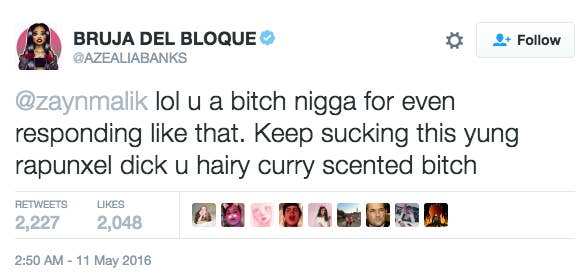
\includegraphics[scale=0.5]{Azealia_banks.jpeg}
  \caption{Azealia Banks tweeting to Zain Malik.}
  \label{fig:azealia_banks}
\end{figure}

The second assumption, that neural models can rely only on the input data and loss functions to identify relevant patterns without the need for human reasoning over the process or the relevance of the input data.
This is lauded as a particular strength of neural network-based machine learning, as it is directed solely by the data without human interference.
Through this data-driven process, models models construct and manipulate their own embodiment, on the basis of the disembodied data with which they are provided.
Moreover, the designers' subjectivities are reflected in the construction and manipulation of the model's embodiment through the designers' decisions surrounding which data to include and how the model is constructed.
In these decisions, the designers also make decisions on which, if any context is necessary to adequately represent the phenomena that is being modelled.
Thus, designers construct and embed the normative values that determine relevance to a task, e.g., abusive language detection.
That is, rather than theoretical or qualitative insights, model weights and probabilistic correlations are emphasised as the appropriate basis for classifications, so long as they reflect the designers' subjectivities.
Such a practice therefore theorises that human cognition is rendered irrelevant by frequentist analyses of words and sub-words.
This (implicit) assumption made by the designers contradicts recent studies that argue that language understanding models do not optimise to the point of having an ability to understand language, instead they optimise to parrot it \citep{Bender-Koller:2020}.

Disregarding for a moment whether such models truly understand language or simply parrot it, what remains clear is that models that only use the surface forms of tokens lay on the globalised end of the model spectrum.
The use of already-optimised language models and word embeddings in a modelling architecture shift the models slightly towards a more localised end of the spectrum, as these allow for some social context to be derived from the way in text is written from a larger data sample.
The use of these pre-optimised technologies thus come to shift the model embodiment away from the embodiments of the users and towards the embodiments of the designers' specific subjectivities.
This shift happens as the choice of which language model and which word embeddings to use is a decision made by the designers.
The decision is made on the basis of which specific pre-optimised technology best aligns with the designers' subjective position on what constitutes abuse and how it is best modelled, i.e. which underlying dataset for these technologies best aligns with the designers' perception of the distinctive features of abuse.

\subsection{Model selection}
As a number of models are optimised to identify which model best embodies the data, the designers must make normative decisions to identify what constitutes `best'.
In this process, designers make a final assertion, embedding their embodiments onto the decision on which model is selected for further use.
However, the choice of designating what constitutes `best' is often times a decision that is made prior to any model optimisation.
For abusive language detection, best often refers to performance for some metrics.
For instance, \citet{Gorrell:2018} set out to have a model that has a high \textit{precision} at the cost of \textit{recall}.
They make this choice to ensure high confidence in their model's predictions of the positive class as their use case is comments made to politicians, where the ability to criticise without sanction is of particular importance.
\citet{Wulczyn:2016} and \citet{Kshirsagar:2018} on the other hand select their models using the Area Under the receiver operating characteristic Curve (AUC) and \textit{F1-score}, respectively.
Both of these metrics for measuring model performance give preference to models that balance classification error types, such that models are attuned to false positives as well as false negatives.

Through the choices of metrics, we can discern some aims of the modelling process.
Where \citet{Gorrell:2018} aim to situate their model within the context of abuse towards British Members of Parliament as it occurs on Twitter, they forego claims of universal applicability.
The best performing model, within their understanding is a model which, within the context, produces as few false positives as possible, explicitly accepting that the number of false negatives may be high.
Considering then the purpose of their modelling process, i.e. to allow for embodied downstream analysis of how abuse targets a very specific group, their choice affords an ability to speak to what is highly likely to be abuse within their understanding of abuse.
On the other hand, their choice does not afford them the ability to speak to what is not abuse nor what their model misclassifies as not being abusive.
\citet{Wulczyn:2016} and \citet{Kshirsagar:2018} on the other hand develop their models with the aim of obtaining a high degree of generalisation onto data outside of the sample that the model is optimised on.
Within this goal lies an assumption that there exist a `universal' and  `objective' understanding of what constitutes abuse, which is invariant to the specific embodiments of different people.
That is, \citet{Wulczyn:2016} and \citet{Kshirsagar:2018} assume the existence of a global understanding of what constitutes abuse for an imagined average user, that is disembodied from all facets of human life.

\section{Dissertation Models}
Here I consider the two model types that I have developed for this dissertation, described in in \autoref{chap:LIWC} and \autoref{chap:mtl}, respectively.
I document the considerations and assumptions that each model type reveals, and its implications for the machine learning pipeline.
Rather than go through the entire pipeline, I begin my analysis at the entry points in the thesis, i.e., the choices of datasets and the modelling choices, as I exclusively use previously published datasets.

\subsection{Vocabulary Reduction}\label{sub:vocab_redux}
In \autoref{chap:LIWC}, I optimised the machine learning models using the datasets published by \citet{Davidson:2017}, \citet{Waseem:2016}, \citet{Waseem-Hovy:2016}, \citet{Wulczyn:2016}, and \citet{Garcia:2018}.
The decision to use these datasets as optimisation data stems from these datasets originating from three distinct sources: Twitter; StormFront, Wikipedia editor discussions; and a white nationalist internet forum, respectively.
To be able to measure the generalisability of the models optimised on \citet{Davidson:2017}, \citet{Waseem:2016}, and \citet{Waseem-Hovy:2016}, I reduce the multi-class classification tasks to binary classification tasks.
Through this reduction in classes, I enforce a normative choice that the detection of abuse has greater value than the identification of the specific type of abuse, e.g., sexism or racism.
My own experiences of hate speech and racialised abuse are at the heart of such a prioritisation, that is having been subject to such abuse I am more concerned with the ability to detect abuse than identifying which specific type of abuse it is.
Further, the modelling choice of how to represent data are also subject to my subjectivities.
While on one hand the reduction of the input space to a much smaller input space means that the size of the subsequent models, and by extension the complexity of the models, is greatly reduced.\footnote{I appreciate that even with a reduction of the model size and complexity, neural networks are still too complex to be readily understood without the aid of additional tools.}
On the other hand, through such a reduction in the vocabulary, a large majority of words will no longer be represented by the text in the models.
Here, my belief that abuse detection models rely to strongly on token occurrences, ultimately impeding the goal of developing models that can protect marginalised people from abuse, is at the centre of my decision.
On the other end of the vocabulary size spectrum, I use byte-pair encoded documents.
Due to the nature of generating sub-words, this increases the size of the vocabulary in comparison to simply using the existing word.
I use sub-words and byte-pair encoding to minimise issues of out-of-vocabulary items which may occur due to intentional obfuscation of words, e.g. through inserting spaces or punctuation in the middle of words \citep{Rottger:2021}.
This is also motivated by my lived experiences and observations of abuse towards others, where peple intentionally obfuscate words to circumvent the simple content filtering techniques, e.g., writing `moslems' instead of `Muslims'.
While the modality I work with is text, such obfuscations also occur in the spoken word through intentional mispronunciation.

In the use of linear models as baseline models, the underlying assumption that I make is is that simple correlations of word occurrences with labels, are insufficient to capture the complex interactions between words that are required to make qualified judgements of abuse.
This assumption too is influenced by my own positionality as a brown Muslim who grew up in a predominately white country where brown people, and in particular Muslims, are vilified for their existence.
One such example were the police bulletins in Danish news while I was growing up.
In these, the description `Muslim looking' were routinely used to describe Brown men.
Such experiences have made it clear to me that social norms surrounding the use of tokens cannot be readily understood from the words using simple correlations without greater contextualisation.
For this reason, I use LSTMs as they can capture long interactions between words and are less directly reliant on the occurrence of individual patterns.
I also use CNNs as a number of past studies having shown the efficacy of CNNs for abuse detection \citep{Park:2017, Mitchell:2019,Kolhatkar:2020,Rizwan:2020,Safaya:2020,Gamback:2017}.

The models described in \autoref{chap:LIWC} that only use words or byte-pair encoded words as input rely entirely on the optimisation data to optimise for patterns in data.
Therefore, those models fall towards the very extreme of the globalised end of the model spectrum.
The models that rely on the LIWC representations, although still on the globalised end of the spectrum, are further towards the localised end, as the LIWC dictionary is informed by considering data that is external to the optimisation data.

The motivation for using Byte-Pair encoding is reflected in a) my own personal assumptions about the importance of textual representations and b) computational considerations.
I use BPE to minimise hte number of out-of-vocabulary items, as BPE deconstructs words in the optimisation data into smaller sub-words.
This deconstruction affords minimising the influence of intentional obfuscations.
Furthermore, the choice to BPE can aid the models in handling unknown tokens better.

Although some of the models are positioned further towards the localised end of the spectrum than others, all the models used in \cref{chap:LIWC} are on the globalised end of the model spectrum.
Their globalised position derives from the fact that none of the data representations take local subjective positionalities of individuals in the data into account.
Instead, all of the models rely on some abstraction away from the self through processes of disembodiment.

\subsection{Multi-Task Learning}\label{sub:mtl_inchap}
In \autoref{chap:mtl} I turn to the question of which constructs, in terms of machine learning tasks, would be helpful for machine learning models to embody to improve performance for a given abusive language detection task.
Specifically, I examine whether jointly learning representations of sarcasm \citep{Oraby_sarcasm:2016}, whether an argument is based in fact or feelings \citep{Oraby_factfeel:2015}, the moral sentiments elicited in tweets \citep{Hoover:2019}, and related notions of hate speech and offensive language \citep{Waseem:2016,Waseem-Hovy:2016,Davidson:2017,Wulczyn:2016} improves classification performance.

For this task, I reuse the BPE representations of documents from \autoref{chap:LIWC}.
Therefore some of the embodiments of the models, with regard to text representation remain the same as described in \cref{sub:vocab_redux}.
Here I focus on the factors from \cref{chap:mtl} that are distinct from \cref{chap:LIWC}.
As I include more datasets into consideration, I also implicitly invite the question `why these datasets'?
To answer this question, it's necessary to revisit the aims of each dataset.

One frequently identified issue with computational modelling of abuse is the issue of sarcasm \citep{Rottger:2021} and I use the dataset labelled for sarcasm that was proposed by \citet{Oraby_sarcasm:2016}.
In this choice lay two assumptions: First, that computational models for abuse detection can benefit from better understanding what constitutes sarcasm.
Second, that there does exist some overlap between sarcasm and abuse, where what appears to be abuse is in fact sarcastic.
Both assumptions are the result of years of researching online abuse, and in particular exposing myself to the abuse that occurs in online spaces.
While I may have become desensitised to abuse through the disproportionate amounts I am exposed to through my research, I frequently see that online abuse, and responses to it are expressed through humour, in particular sarcasm.\footnote{By responses I mean general reactions and responses to abuse beyond the direct responses to a perpetrator of abuse.}

The second dataset, asks the question of whether an argument is made in the basis of feeling or on the basis of facts \citep{Oraby_factfeel:2015}.
As a majority of people who perpetrate online abuse do so infrequently \citep{Waseem-Hovy:2016}, an underlying cause for being abusive may be being impassioned, and thus being able to determine whether an argument is made with a basis in feelings or fact may be possible to help improve performance for abuse detection.

I also use a dataset annotated for moral foundation \citep{Hoover:2019}.
In this dataset, each document is labelled for which moral foundations it invokes in the annotators.
Moral foundations and online abuse can be thought of as orthogonal concepts.
Moral foundations, as annotated in the dataset, provide for a higher level cognition about the content that is read, in which abusive content is likely to elicit the moral sentiments that comprise the moral foundations framework \citep{Hoover:2019}.
I therefore believe that machine learning models jointly embodying abuse and moral foundations can aid with improving performance of machine learning classifiers for abuse detection.
My own experiences of racialised abuse and observations of abuse in online spaces combined with the apparent desire of abusers to inflict harm upon their target are central to my inclusion of this task.

Finally, I use a number of datasets for online abuse \citep{Garcia:2018,Waseem:2016,Waseem-Hovy:2016,Davidson:2017,Wulczyn:2016}.
For this task, I do not reduce the question of detecting to a binary task, instead I use the auxiliary task datasets as a means to provide the model with more conceptualisations of abuse.
However, my subjective positioning does not change from what is detailed in \autoref{sub:vocab_redux}.

Similarly for the choices in developing the data and textual representations, my own subjective embodiments and experiences are a key factor in the modelling decisions (see \cref{sub:vocab_redux}).
This is particularly true for MTL, where I specifically set the weights for how much each task is to contribute to the main task through the frequency of selection.
Such a weighting relies on my own consideration of how important each task is to the overall task of identifying abuse and, subsequently, the degree to which each auxiliary task should be afforded space to influence the model representations for abuse.
The specific architecture of the model is influenced by its usefulness in prior work \citep{Bingel:2018} in addition to seeking an to answer the question of how more complex models would influence the performance on the task.

Using the MTL framework has strong implications for where on the localisation spectrum the model is positioned.
For instance, the use multiple different datasets to influence a single model precludes the extreme ends of the modelling spectrum.
Jointly optimising multiple tasks in a shared internal model layer explicitly shifts models away from the extreme of the globalised spectrum, by providing using datasets that are external to the main task dataset and by contextualising the main task with the representations obtained from the auxiliary tasks.
Similarly, the localised extreme of the model spectrum is also precluded using this method, as the auxiliary tasks do not afford embedding the subjectivities and embodiments of individuals.
On a demographic level, however, MTL does hold potential for shifting towards the localised extrema, if and only if all auxiliary tasks also come from the demographic that the main task is concerned with.
Moreover, as each auxiliary task will work, if as nothing else, as a regulariser for the main task, MTL will shift the model away away from the extremes of the spectrum.
In my use of MTL for abusive language detection, with the auxiliary tasks that I have chosen, the models that I have developed are shifted away from the globalised extrema towards a more localised position on the model spectrum.
However, as I do not optimise my models on any tasks that seek to make predictions on users, and the distinct datasets do not originate from the same demographic, the model remains a globalised model.
Instead the models that I produce, by virtue of learning considerations on tone, argument basis, sarcasm, and moral sentiment, optimise for some representations of the faculties that I believe of importance to the task.
These auxiliary tasks then provide an avenue for the models to be more closely situated within the how each individual person can be represented as a function of how they express themselves.
Thus, while further towards being a localised end of the spectrum than the LIWC models, the models fall short of significantly situating the modelling of individuals within the context and lived experiences of that individual.

\section{Discussion}
Given that subjective choices and biases masquerading as disembodied `objective' positions permeate the machine learning pipeline, the quest for objectivity and bias-free machine learning becomes redundant.
This redundancy is made apparent as all choices in the machine learning development pipeline embody the subjective experiences of all who are a part of the pipeline, from the people whose data is seized, to annotators and the designers of the pipelines.
As these experiences are embedded in the system, so slips away the illusion of `objectivity' and `neutrality' of the machine learning technologies.
In fact, the search for objectivity in the pipeline creates a veneer of social progress that may cause further harm to already marginalised communities by obscuring and entrenching the dominance of certain bodies over others.
Such harm is instituted by providing a veneer of more just, or fair, machine learning technologies that nonetheless perform institutional violence upon all who are externalised by the development process and the subjective experiences that lie at the heart of them.
Without taking the unique embodiments of all data subjects into account, this imaginary of fair only serves as a justification of maintaining oppressive structures that are inherently harmful and reductive.

Considering the task of hate speech detection, developing automated tools, that are applied to a general population, makes inherent decisions on behalf of the user-group.
The decisions made by the third party adjudicator, i.e. content moderation technologies, embed subjective experiences of the data subjects whose data has been stripped from the context it was created in, the annotators, and the designers of the technologies.
Such decisions are codified through the machine learning pipeline, and are presented as disembodied and objective decisions on what constitutes hate speech.
In this way, machine learning technologies embed normative socio-political positions on respectability and acceptability.
These normative values come to be presented as `objective' through the disembodiments that occur in the machine learning pipeline.
However, such notions of objectivity merely provide a thin veil over the subjective embodiments of the designers and annotators.
With the vast majority of research on abusive language detection being developed for English in the global north \citep{Vidgen-Derczynski:2020}, the notions of respectability that are embedded in the technologies are normative for white majoritarian countries and cultures.
Through such codification of white perspectives on respectability masqueraded as objective, attempts to address `bias' in machine learning technologies for content moderation only serve to justify existing oppressive structures by further obscuring the subjectivities and norms embedded in the systems.

A consideration of how data is embodied can empower designers of machine learning systems by allowing them to reflect on what is embodied and how it is mired in context.
Such considerations allow designers to interrogate the contexts within which data are created, and how meaning is made at each step in the dataset creation process.
It is through such recognition of context and embodiment that one can realise that as contexts change, so does the applicability data.
Further, only by such recognition of the deeply complex nature of embodiment and data can one hope to ask and ascertain which views the models privilege and which are subjugated.
For building content moderation systems for the detection of hate speech and abuse, the designers of machine learning pipelines can ask how their own embodiments prejudice them to selectively sanction some speech patterns.
Moreover, designers may want to ask themselves how such sanctions create downstream implications for the speech that is sanctioned.

Although there are methods with which we can move towards more localised machine learning models, what positions are given space remains a political question.
It is only through wholly representing the context and embodiments of the data creator and the datum that one can hope to arrive at sufficiently localised models.
Thus, rather than asking how to eliminate bias and subjective experiences from machine learning in the pursuit of objectivity, shifting the question to consider embodiments would ask us to reflect on the subjective experiences that are given voice.
For hate speech detection, such reflections would have designers ask which groups understandings of abuse it is most appropriate to ground their definitions, and subsequently annotations and models, in.
Such a shift would then require us to ask and reflect upon which bodies' subjective experiences we need to account for, such that we give voice to socially, and computationally marginalised groups.

Only by recognising the positionality of the designers and annotators of machine learning models and data, can one account for what (and whom) ones own position, and the models derived from it privilege and sanction, give space for and the political ramifications of this.
For these reasons, it is imperative that machine learning moves away from consolidating power in the designers and move towards development practices that are rooted in the participation of the people who will be subject to the models, i.e. the intended users of the models.
Participatory design practices however can quickly turn predatory if the turn to participatory design principles does not also provide for a redistribution of power \citep{Kelly_2019}.
Here, Sasha Costanza-Chock's \citeyearpar{Costanza-Chock_2018} work on design justice can provide a guide towards developing participatory design practices for machine learning.
\citet{Costanza-Chock_2018} argues for design practices that centre the experiences and needs of the communities for whom the design practice is taking place.
Specifically, \citet{Costanza-Chock_2018} argues that design practices should have ``sustainable, community-led and -controlled outcomes.''
By working towards such goals, machine learning research can come develop processes and technologies that specifically address the needs of the communities for whom we are developing our technologies.

\section{Summary}
In this chapter, I have sought to examine how subjective embodiments permeate the machine learning pipeline, in efforts examine the machine learning infrastructures that underpin contemporary content moderation technologies.
Thus, in this chapter I seek to examine \textit{RQ I} by examining how subjective embodiments are embedded into machine learning infrastructures and what the consequences of such embodiments are.
In this chapter, I then provide a reading of machine learning against the grain by critically examining how subjective embodiments become embedded within the machine learning infrastructure.
By performing this reading, I have used this chapter to examine the ways in which machine learning systems come to produce socially biased outcomes, such that machine learning research can move beyond the discriminatory practices that we have developed.

Identifying processes for developing machine learning technologies that are not discriminatory, is of particular importance to content moderation technologies, as these technologies currently produce discriminatory outcomes in terms of censorship of marginalised communities (see \cref{chap:filter} for further details).
The work that I have performed in this chapter, identifies specific ways in which machine learning, and machine learning for content moderation encodes the subjectivities that are widely read as social biases.
To address this concern, I propose that researches be aware of the specific ways in which they embed their subjectivities throughout the machine learning pipeline and consciously make decisions in the development process that ensure that the subjectivities that are embedded within the systems reflect the aims and the subjectivities of the people that the content moderation systems are to be applied to.
Specifically, I suggest that researchers are mindful of their own subjectivities and the desired outcomes of the technologies, and that research engages in a genuine efforts for participatory design by collaborating with the communities that technologies are developed for.
Moreover, I argue that the universalist notions applied in machine learning, including the algorithmic detection of abusive language, contribute strongly to the ongoing marginalisation that machine learning systems perpetuate.
Finally, I argue that it is only by taking steps away from such universalist notions and towards co-developing systems with communities that are community-led and community-controlled that we can hope to overcome the issues of discriminatory systems and, in the case of content moderation, systems that do not censor marginalised communities.
%
% \section{Machine Learning as a Conservative Practice}
% \zw{Write about dominant and subjugated discourses for machine learning here; bring in that ML is a conservative practice}
%
% \zw{Citations needed: Foucault on dominant and subjugated discourses, Fraser on subaltern publics, some archival theory on marginalising effects of dominant discourses.i}

